\documentclass[11pt]{article}
\usepackage[margin=1in]{geometry}
\usepackage{booktabs}
\usepackage{longtable}
\usepackage{array}
\usepackage{graphicx}
\usepackage{hyperref}
\graphicspath{{./memo_11_figures/}{Memory/memo_11_figures/}}

\title{Memo 11: Case B Node/Core Speed-Test Matrix and Timing Analysis}
\author{FVCOM-MP WaterPACT Investigation}
\date{May 2026}

\begin{document}
\sloppy
\setlength{\tabcolsep}{4pt}
\maketitle

\section*{Purpose}

This memo defines a compact speed-test matrix for case B on Kestrel and
summarizes the observed timing analysis.  The goal is to estimate the present
one-class FVCOM-MP runtime sensitivity to MPI rank count and node placement.
The observed SEC/IT values, speedup calculations, and plots have been moved to
\texttt{Analysis/analyze\_memo\_11\_speed.py} so the analysis can be rerun
without hand-editing the memo.

The current case-B run script uses:
\begin{itemize}
  \item case name: \texttt{waterPACT\_b};
  \item run directory: \texttt{FVCOM\_MP\_test\_run/RUN\_b};
  \item plastic input: \texttt{generic\_plastic\_b.inp};
  \item sediment input: \texttt{mp\_sediment\_a\_no\_adv.inp};
  \item current production-style Slurm layout: \texttt{nodes=4},
        \texttt{ntasks-per-node=104}, total MPI ranks = 416.
\end{itemize}

Kestrel nodes are assumed to allow up to 104 MPI ranks per node for this test.
The table below starts from one core, expands through useful within-node and
across-node configurations, and then adds a C-series extension to search for
the maximum practical long-run speedup.

\section*{Primary Speed-Test Matrix}

\footnotesize
\begin{longtable}{l>{\raggedright\arraybackslash}p{1.25in}rrr>{\raggedright\arraybackslash}p{2.05in}}
\caption{Recommended case-B speed-test combinations.}\\
\toprule
Run ID & Scaling role & Nodes & Tasks/node & Total ranks & Purpose \\
\midrule
\endfirsthead
\toprule
Run ID & Scaling role & Nodes & Tasks/node & Total ranks & Purpose \\
\midrule
\endhead
\bottomrule
\endfoot
B01 & single-core baseline & 1 & 1 & 1 & Absolute serial-like MPI baseline. \\
B02 & small within-node & 1 & 2 & 2 & First parallel efficiency point. \\
B03 & small within-node & 1 & 4 & 4 & Early scaling slope. \\
B04 & small within-node & 1 & 8 & 8 & Useful low-cost debug point. \\
B05 & medium within-node & 1 & 16 & 16 & Checks communication overhead onset. \\
B06 & medium within-node & 1 & 32 & 32 & Mid-node scaling. \\
B07 & half node & 1 & 52 & 52 & Half of one 104-core node. \\
B08 & dense within-node & 1 & 64 & 64 & Common power-of-two-ish reference below full node. \\
B09 & dense within-node & 1 & 78 & 78 & Three-quarter node occupancy. \\
B10 & full node & 1 & 104 & 104 & Maximum single-node occupancy. \\
B11 & spread-vs-pack check & 2 & 52 & 104 & Same total ranks as B10, but spread across two nodes. \\
B12 & two full nodes & 2 & 104 & 208 & First full multi-node test. \\
B13 & spread-vs-pack check & 4 & 52 & 208 & Same total ranks as B12, but spread across four nodes. \\
B14 & three full nodes & 3 & 104 & 312 & Intermediate full-node scaling. \\
B15 & current full setup & 4 & 104 & 416 & Matches the present case-B production-style layout. \\
B16 & eight-node spread check & 8 & 52 & 416 & Same total ranks as B15, but spread across eight nodes. \\
B17 & dense eight-node test & 8 & 78 & 624 & Intermediate eight-node occupancy. \\
B18 & full eight-node test & 8 & 104 & 832 & Maximum eight-node occupancy. \\
B19 & full five-node test & 5 & 104 & 520 & Checks whether full-node scaling continues past B15. \\
B20 & full six-node test & 6 & 104 & 624 & Same total ranks as B17, but packed into six full nodes. \\
B21 & full seven-node test & 7 & 104 & 728 & Near-eight-node full scaling point. \\
B22 & six-node spread check & 6 & 70 & 420 & Similar rank count to B15/B16, spread over six nodes. \\
C01 & ten-node spread check & 10 & 52 & 520 & Same total ranks as B19, but spread over ten nodes. \\
C02 & ten-node moderate occupancy & 10 & 64 & 640 & Near the B17/B20 rank count with lower per-node occupancy. \\
C03 & ten-node dense occupancy & 10 & 78 & 780 & Extends the best observed 78 ranks/node occupancy beyond eight nodes. \\
C04 & twelve-node spread check & 12 & 52 & 624 & Same total ranks as B17/B20, but spread over twelve nodes. \\
C05 & twelve-node moderate occupancy & 12 & 64 & 768 & Moderate twelve-node scaling point. \\
C06 & twelve-node dense occupancy & 12 & 78 & 936 & Tests whether the B17 occupancy remains favorable past eight nodes. \\
C07 & sixteen-node spread check & 16 & 52 & 832 & Same total ranks as B18, but spread over sixteen nodes. \\
C08 & sixteen-node moderate occupancy & 16 & 64 & 1024 & Clean 1024-rank test for higher maximum speedup. \\
C09 & sixteen-node dense occupancy & 16 & 78 & 1248 & Main candidate for a new maximum-speed configuration. \\
C10 & sixteen-node full occupancy & 16 & 104 & 1664 & Diagnostic full-node test; checks whether full occupancy remains slower. \\
\end{longtable}
\normalsize

\section*{Priority Subset for Debug Queue}

If the debug queue time or node limit is tight, the minimum useful subset is:
\begin{center}
\begin{tabular}{lrrr}
\toprule
Run ID & Nodes & Tasks/node & Total ranks \\
\midrule
B01 & 1 & 1 & 1 \\
B04 & 1 & 8 & 8 \\
B06 & 1 & 32 & 32 \\
B10 & 1 & 104 & 104 \\
B12 & 2 & 104 & 208 \\
B15 & 4 & 104 & 416 \\
B16 & 8 & 52 & 416 \\
B20 & 6 & 104 & 624 \\
B22 & 6 & 70 & 420 \\
B18 & 8 & 104 & 832 \\
\bottomrule
\end{tabular}
\end{center}

This subset gives one single-core anchor, three within-node scaling points, and
four multi-node points.  If only one 8-node job is practical, keep B16 because
it directly compares against B15 at the same total rank count.

\section*{Suggested Slurm Fields to Change}

For each speed test, change only the Slurm resources and job name:
\begin{verbatim}
#SBATCH --partition=debug
#SBATCH --nodes=<Nodes>
#SBATCH --ntasks-per-node=<Tasks/node>
#SBATCH --job-name=WFPb_<Run ID>
\end{verbatim}

Keep the executable command unchanged:
\begin{verbatim}
srun ./fvcom_TLMF --casename=waterPACT_b
\end{verbatim}

For clean comparisons, use the same executable, same input files, same output
settings, and same initial condition for every run.  The speed-test output can
be stored in separate Slurm log files; full NetCDF output is not needed if the
debug run is only long enough to capture representative per-step timing.

\section*{Automated Timing Analysis}

The raw observed timing table is no longer maintained inside this memo.  To
regenerate the SEC/IT plot, speedup plot, key comparison tables, and written
interpretation, run:
\begin{verbatim}
python Analysis/analyze_memo_11_speed.py
\end{verbatim}
from the repository root.  The script writes the generated figures and the
LaTeX analysis block included below.

\IfFileExists{memo_11_speed_analysis.tex}{%
  % Auto-generated by Analysis/analyze_memo_11_speed.py.
% Do not edit this file directly; update the Python timing data and rerun.

\subsection*{Observed Timing Results}

The observed SEC/IT values are stored in \texttt{Analysis/analyze\_memo\_11\_speed.py}.
That script computes the speedup relative to B01, parallel efficiency, same-rank
spread/pack comparisons, and the figures below.

\begin{figure}[htbp]
\centering
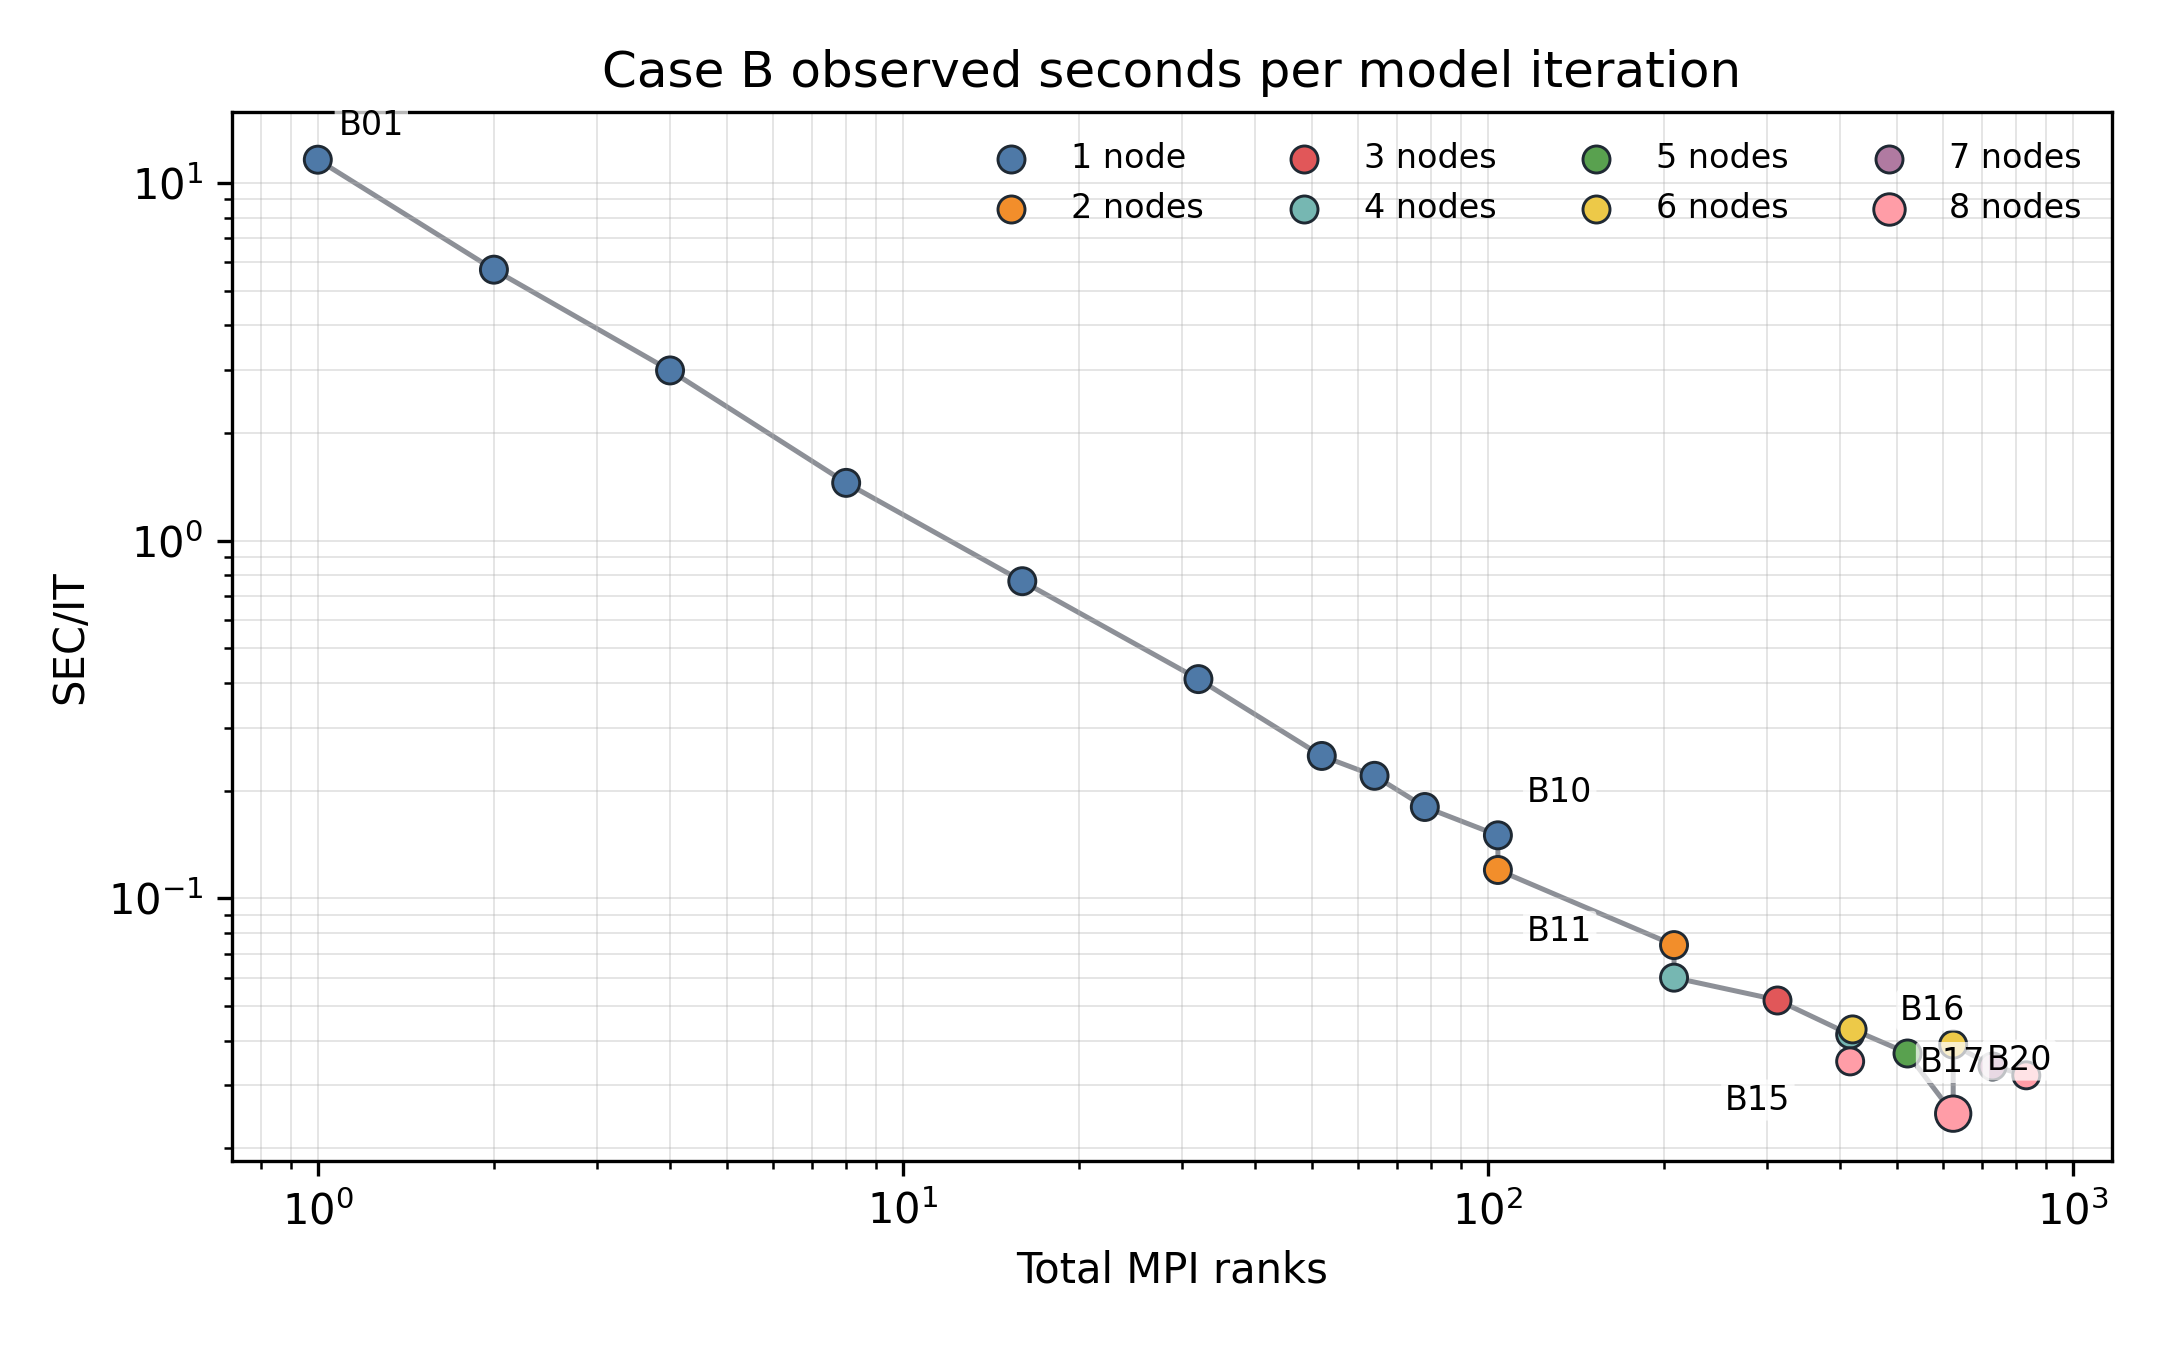
\includegraphics[width=0.92\linewidth]{memo_11_sec_per_iteration.png}
\caption{Observed case-B SEC/IT versus total MPI ranks. Lower values are faster; B17 is the fastest observed point.}
\end{figure}

\begin{figure}[htbp]
\centering
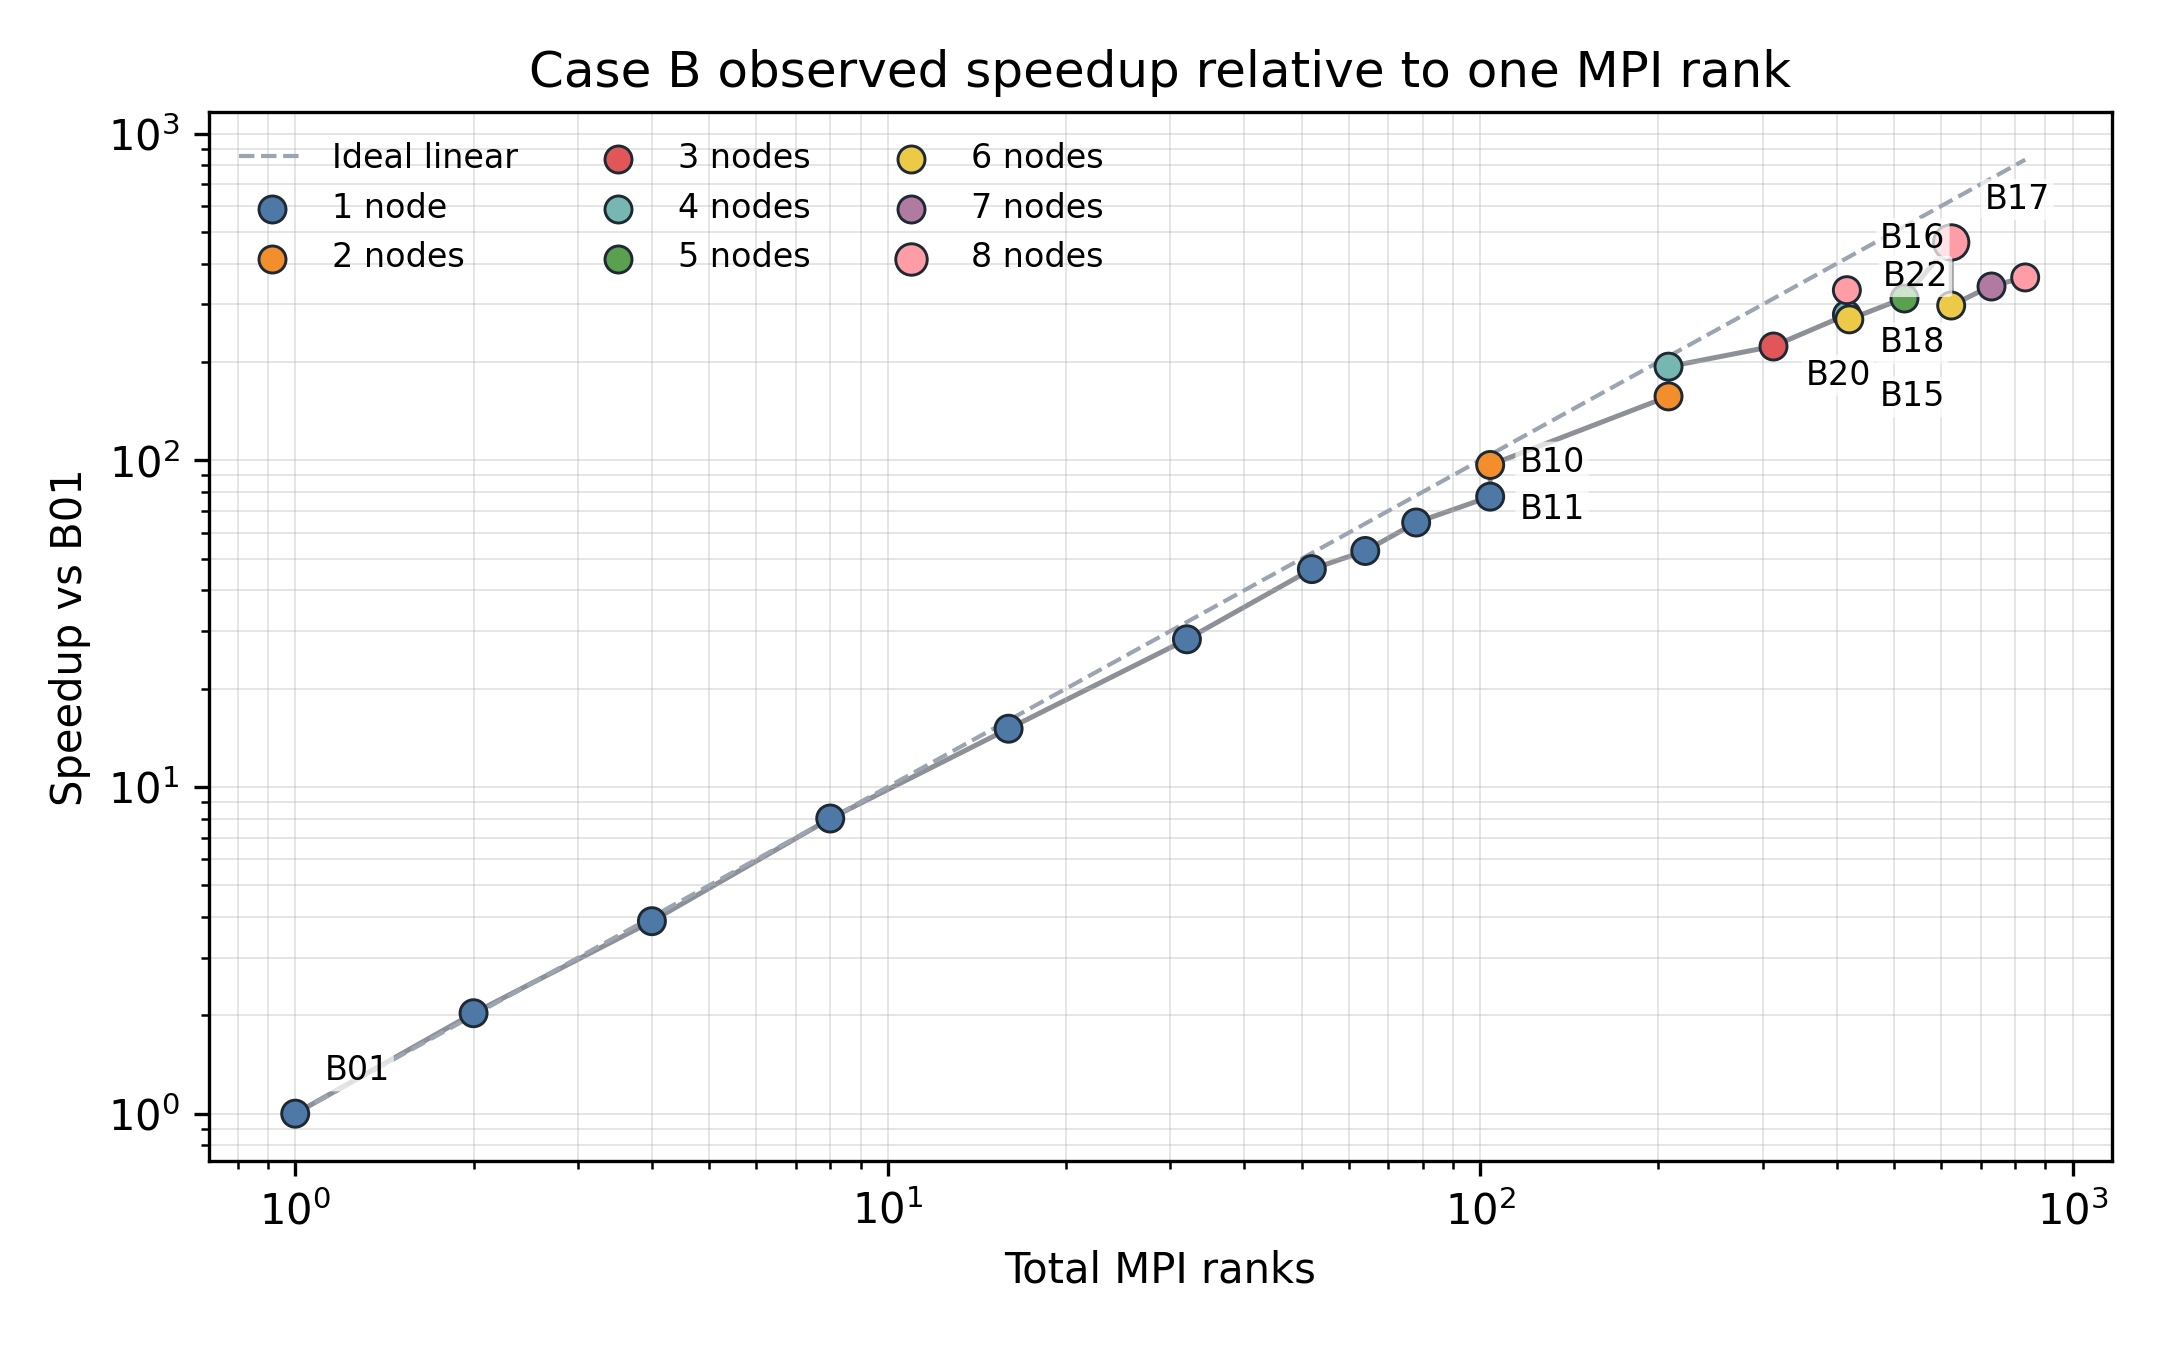
\includegraphics[width=0.92\linewidth]{memo_11_speedup.png}
\caption{Observed speedup relative to the B01 one-rank baseline. The dashed line marks ideal linear speedup.}
\end{figure}

\begin{table}[htbp]
\centering
\caption{Key observed timing configurations generated from the analysis script.}
\begin{tabular}{lrrrrr}
\toprule
Run ID & Layout & Ranks & SEC/IT & Speedup & Efficiency \\
\midrule
B15 & 4 x 104 & 416 & 0.0416 & 279.1 & 67.1\% \\
B16 & 8 x 52 & 416 & 0.035 & 331.7 & 79.7\% \\
B17 & 8 x 78 & 624 & 0.025 & 464.4 & 74.4\% \\
B18 & 8 x 104 & 832 & 0.032 & 362.8 & 43.6\% \\
B20 & 6 x 104 & 624 & 0.039 & 297.7 & 47.7\% \\
\bottomrule
\end{tabular}
\end{table}

\begin{table}[htbp]
\centering
\caption{Same-rank or near-diagnostic node-spread comparisons.}
\begin{tabular}{llll}
\toprule
Rank case & Packed/reference & Spread/candidate & SEC/IT change \\
\midrule
104 ranks & B10, 1 x 104 & B11, 2 x 52 & 20.0\% faster \\
208 ranks & B12, 2 x 104 & B13, 4 x 52 & 18.9\% faster \\
416 ranks & B15, 4 x 104 & B16, 8 x 52 & 15.9\% faster \\
624 ranks & B20, 6 x 104 & B17, 8 x 78 & 35.9\% faster \\
\bottomrule
\end{tabular}
\end{table}

\subsection*{Analysis Interpretation}

The fastest observed configuration is \textbf{B17}, with
8 nodes, 78 ranks per node,
624 total ranks, and 0.025 SEC/IT.
This is a 464.4x speedup over B01 and is
39.9\% faster than the current four-node B15 layout.

For the near-416-rank operating point, \textbf{B16} is the
best observed choice: 0.035 SEC/IT compared with
0.0416 SEC/IT for B15.  The matched-rank checks show
that spreading ranks across more nodes improves timing for 104, 208, 416, and
624 total ranks in these observations.

The eight-node full-occupancy run B18 is slower than B17 by
28.0\%, even though B18 uses more ranks.  This suggests that
the present sweet spot is not maximum rank count, but moderate per-node
occupancy on eight nodes.  The practical recommendation is to use B17 when the
queue allows eight nodes, use B16 for a 416-rank comparison run, and repeat
B16--B18 if final production timing needs tighter uncertainty bounds.

}{%
  \noindent Generated timing analysis is missing. Run
  \texttt{python Analysis/analyze\_memo\_11\_speed.py} from the repository
  root and rebuild this memo.
}

\end{document}
